\begin{center}
{\textbf{Lundi 16 août 2021 : L’aventure commence}}
\end{center}
\vspace{2mm}

Centre International de Valbonne, 33° Celsius. Arrivant de tous les recoins de la France (et au-delà), les stagiaires rejoignent peu à peu le campus. Les plus studieux s’attaquent sans délai à la grande Muraille d’exercices, d’autres commencent avec engouement les premières parties de cartes de la saison.

\begin{figure}[H]
\centering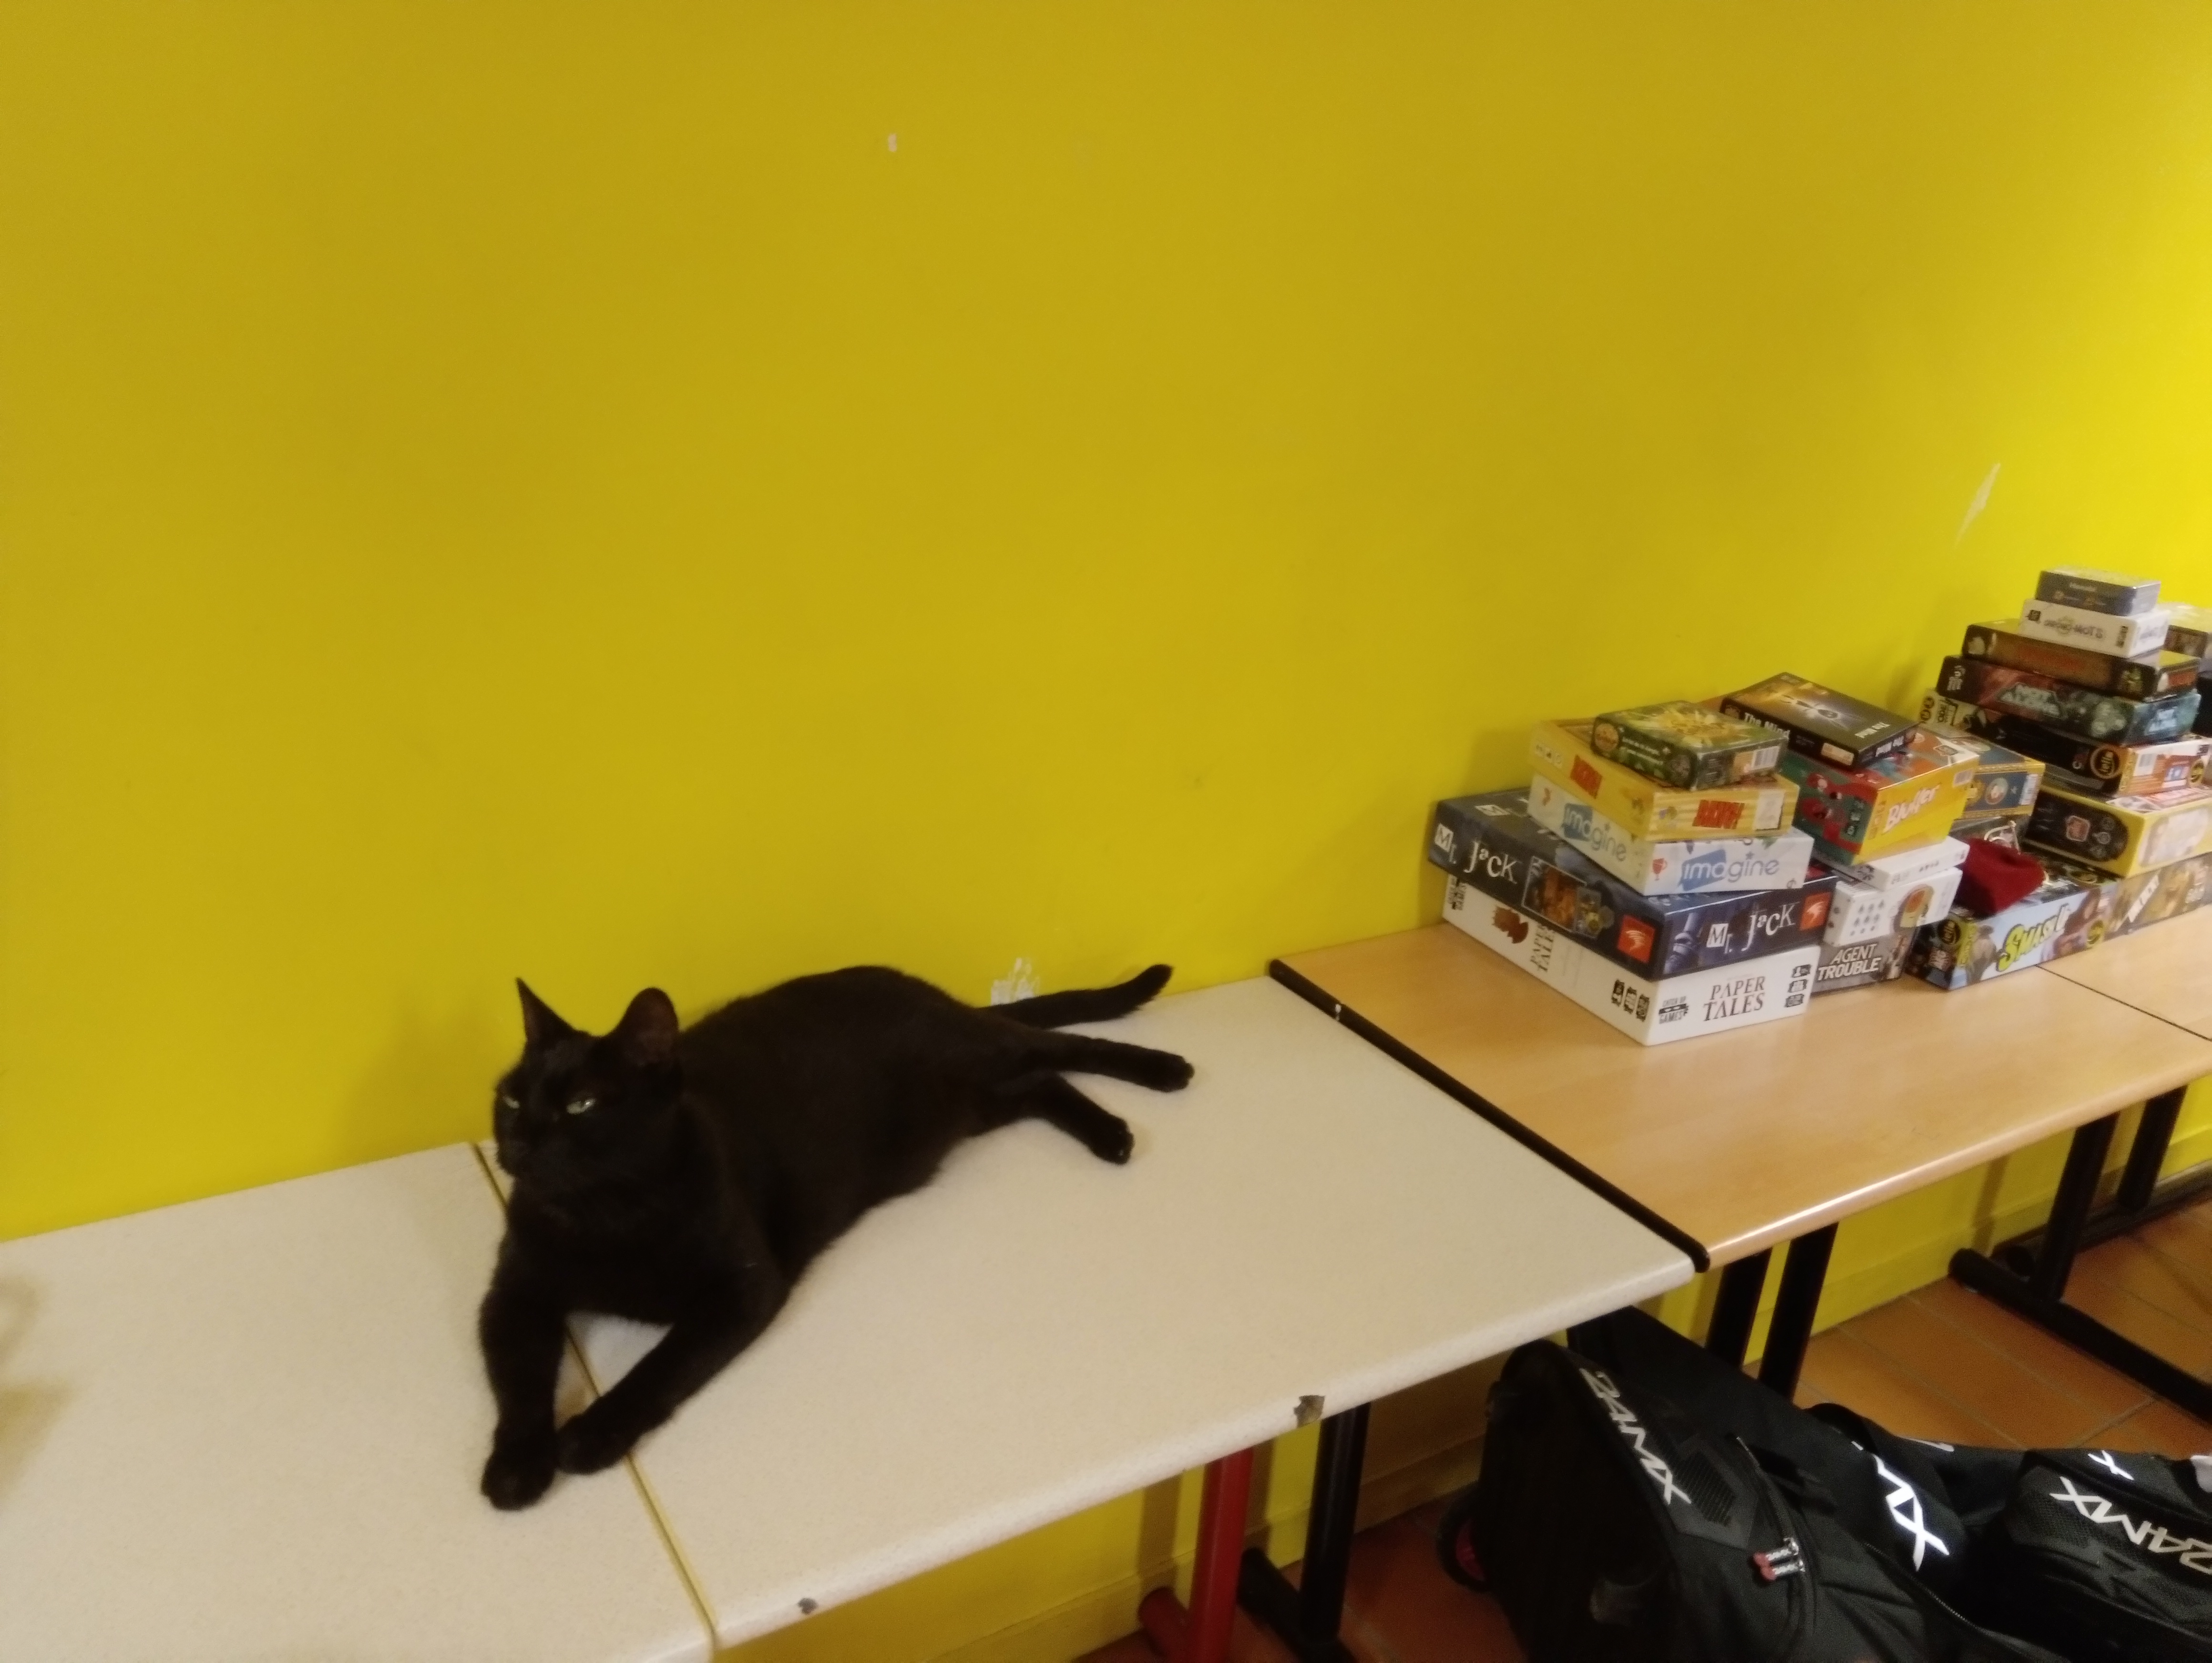
\includegraphics[width=6cm]{CR-16-0.jpg}
\caption{Personne ne remarque un imposteur sournois introduit parmi les participants…}
\end{figure}

Les activités sont brièvement interrompues par un petit questionnaire suivi d’un court entretien pour la constitution des groupes : collégiens débutants (A), lycéens débutants (B), élèves avec déjà une certaine expérience des mathématiques olympiques (C) et élèves avancés (D). Les animatheurs tentent de juguler l’insatiable soif de connaissance des élèves, qui souhaitent rejoindre les groupes les plus avancés. Mais que peuvent-ils faire contre leur volonté de fer et leur enthousiasme débordant ?

À 20 h, il est enfin temps de procéder aux rituels traditionnels de la première soirée. Une fois tout le monde rassemblé dans l’amphithéâtre, les élèves font la connaissance avec les animatheurs présents en ce début de stage. Puis, Théo, reprenant le flambeau (ainsi que les diapositives) de Vincent, livre avec entrain et bonne humeur une présentation des olympiades mathématiques et de la POFM. Et évidemment, la réunion se clôt avec remise des prix aux gagnants de la coupe Animath.

\begin{figure}[H]
\centering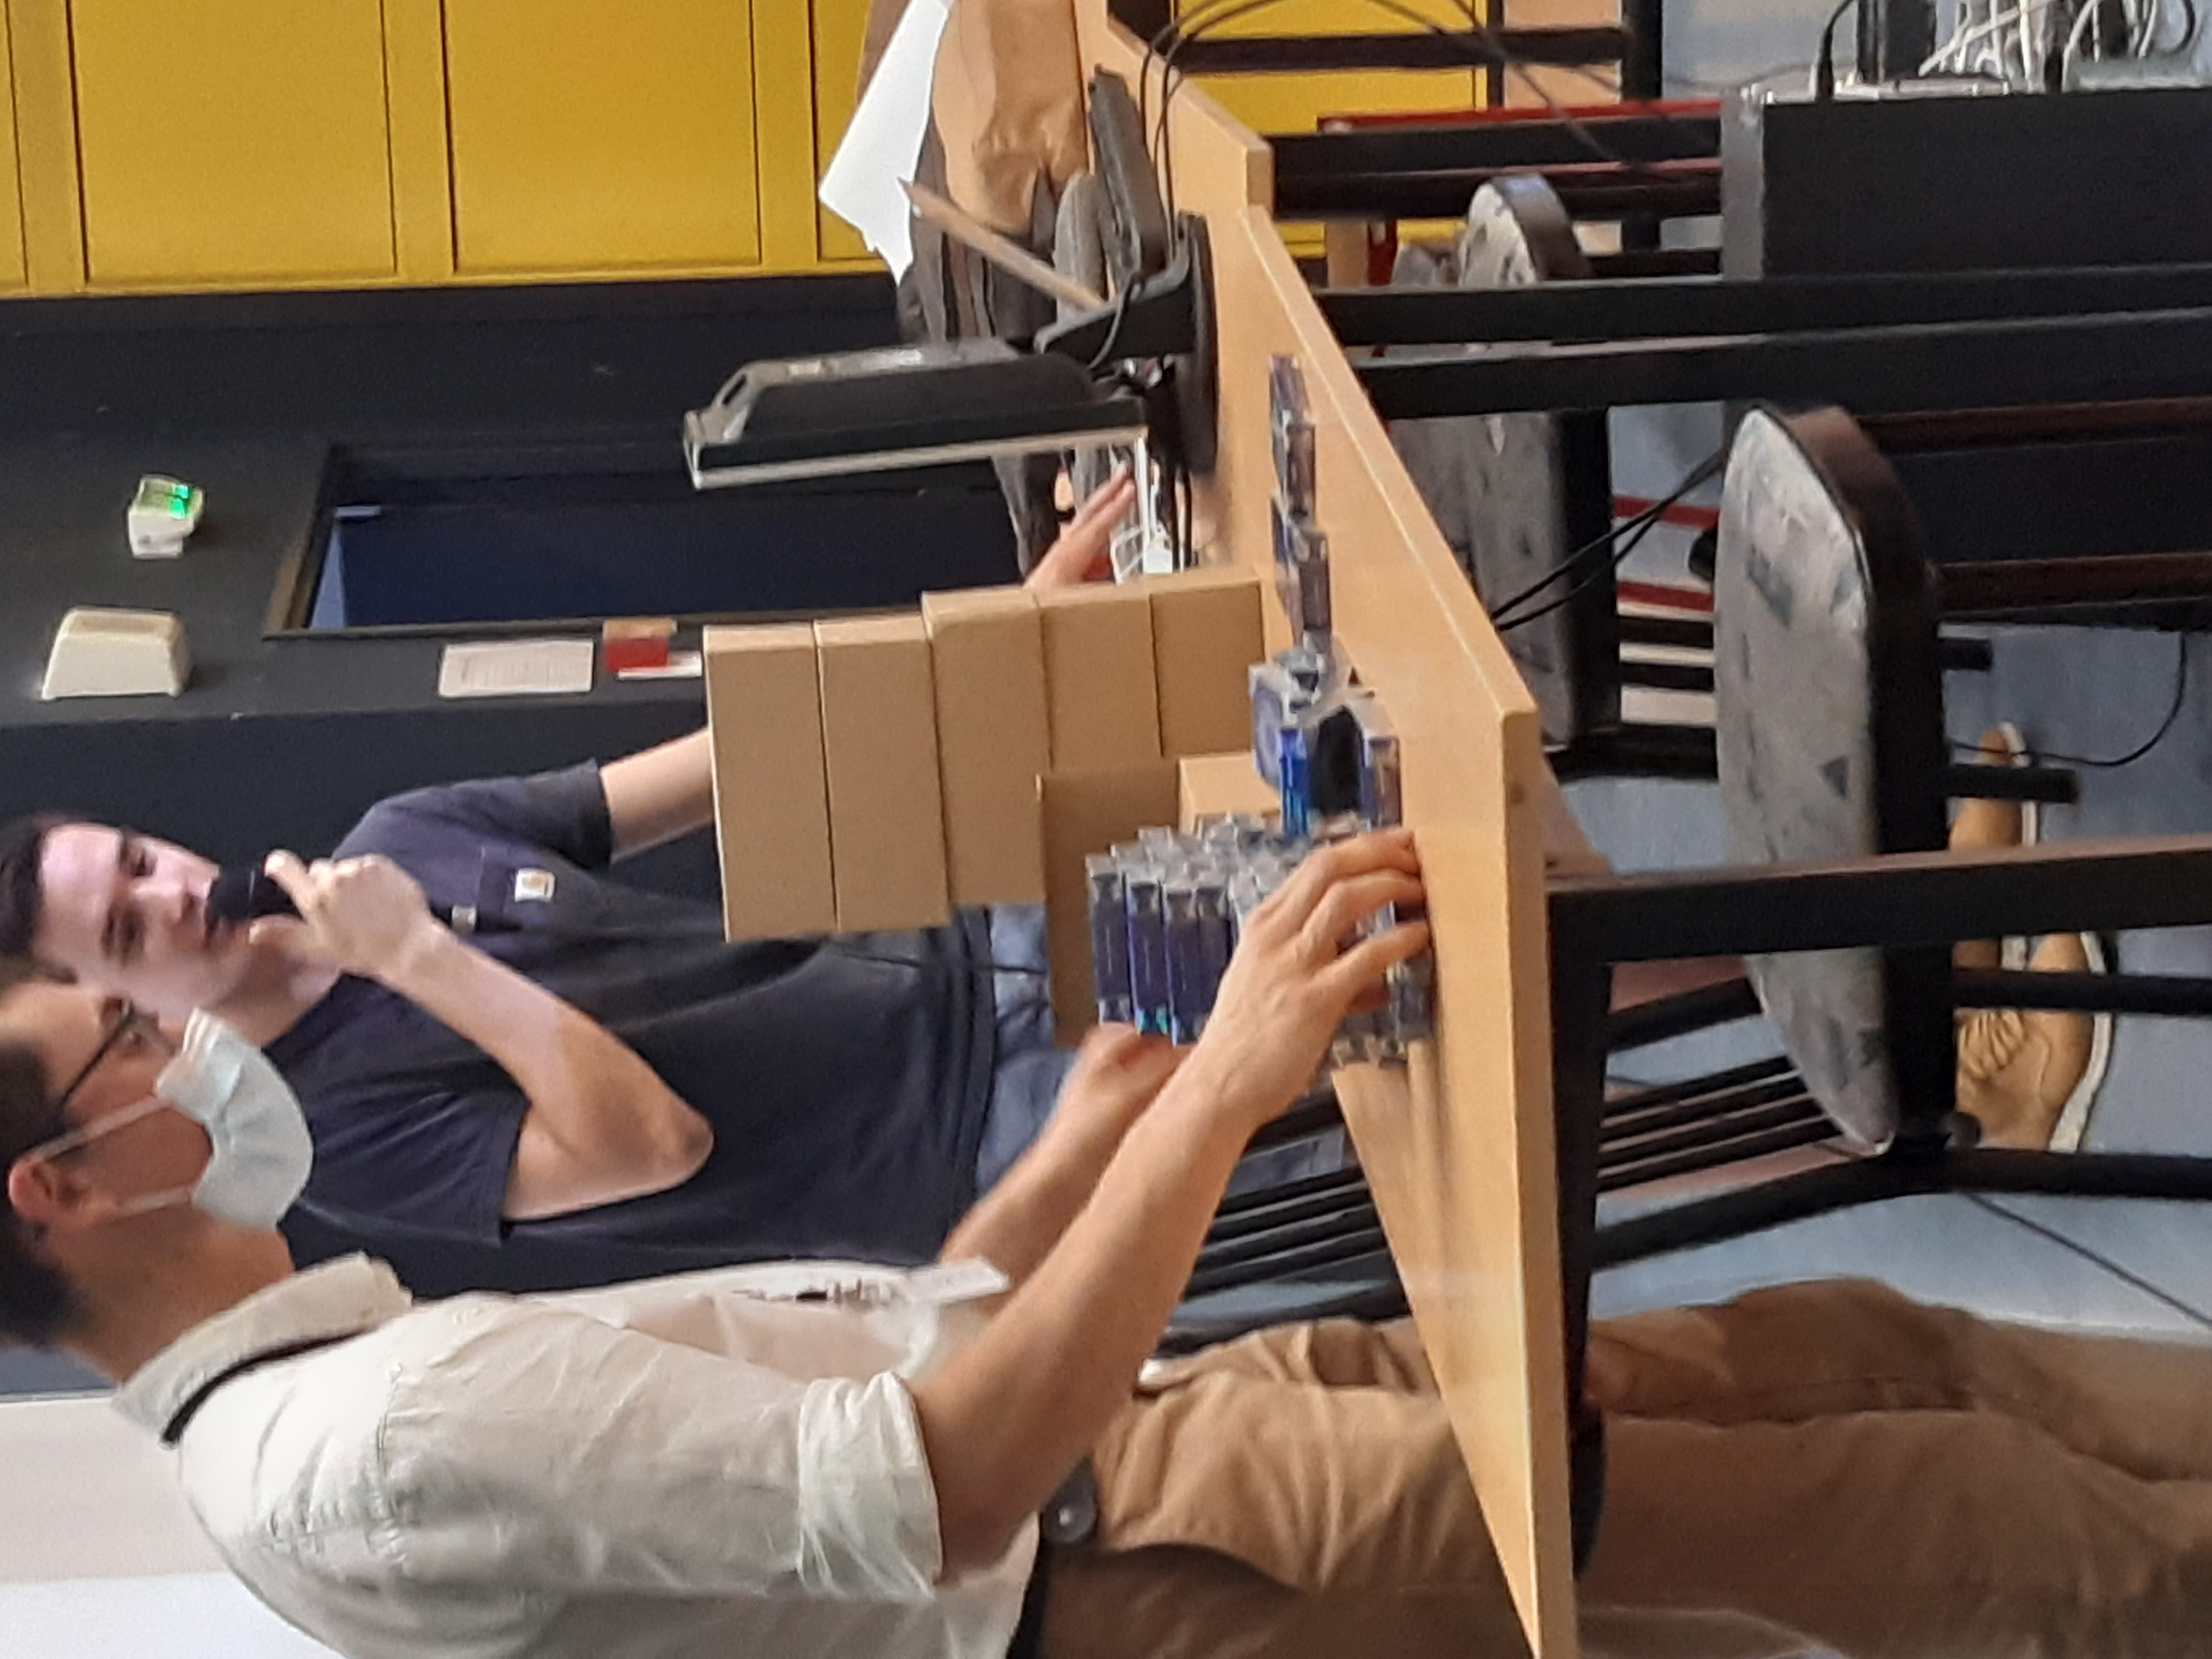
\includegraphics[width=6cm]{CR-16-1.jpg}
\caption{De gauche à droite : Gaëtan Dautzenberg, George Tézé, Auguste Ramondou, Henri Hovasse, et Pierre Akin Dürrüoglu}
\end{figure}


Le lecteur averti remarquera qu’il manque un détail. En effet, qu’en est-il donc de la couleur des nouveaux T-shirts Animath? Hélas, ce n’est pas ce soir que les parieurs impatients auront la réponse, car le colis si convoité n’est pas encore arrivé. En attendant, les participants doivent se contenter d’un T-shirt Jane Street, nouveau généreux sponsor d’Animath.

Après les péripéties de la première journée, les élèves peuvent échanger la chaleur quelque peu étouffante de l’amphi contre l’air frais du soir. On se disperse pour profiter de divers jeux de société, ou bien d’un repos bien mérité.